%%%%%%%%%%%%%%%%%%%%%%%%%%%%%%%%%%%%%%%%%
% Short Sectioned Assignment
% LaTeX Template
% Version 1.0 (5/5/12)
%
% This template has been downloaded from:
% http://www.LaTeXTemplates.com
%
% Original author:
% Frits Wenneker (http://www.howtotex.com)
%
% License:
% CC BY-NC-SA 3.0 (http://creativecommons.org/licenses/by-nc-sa/3.0/)
%
%%%%%%%%%%%%%%%%%%%%%%%%%%%%%%%%%%%%%%%%%

%----------------------------------------------------------------------------------------
%	PACKAGES AND OTHER DOCUMENT CONFIGURATIONS
%----------------------------------------------------------------------------------------

\documentclass[paper=a4, fontsize=11pt]{scrartcl} % A4 paper and 11pt font size

\usepackage[T1]{fontenc} % Use 8-bit encoding that has 256 glyphs
\usepackage{fourier} % Use the Adobe Utopia font for the document - comment this line to return to the LaTeX default
\usepackage[english]{babel} % English language/hyphenation
\usepackage{amsmath,amsfonts,amsthm} % Math packages
\usepackage[pdftex]{graphicx}
\graphicspath{{./}}

\usepackage{lipsum} % Used for inserting dummy 'Lorem ipsum' text into the template

\usepackage{sectsty} % Allows customizing section commands
\allsectionsfont{\centering \normalfont\scshape} % Make all sections centered, the default font and small caps

\usepackage{fancyhdr} % Custom headers and footers
\pagestyle{fancyplain} % Makes all pages in the document conform to the custom headers and footers
\fancyhead{} % No page header - if you want one, create it in the same way as the footers below
\fancyfoot[L]{} % Empty left footer
\fancyfoot[C]{} % Empty center footer
\fancyfoot[R]{\thepage} % Page numbering for right footer
\renewcommand{\headrulewidth}{0pt} % Remove header underlines
\renewcommand{\footrulewidth}{0pt} % Remove footer underlines
\setlength{\headheight}{13.6pt} % Customize the height of the header

\numberwithin{equation}{section} % Number equations within sections (i.e. 1.1, 1.2, 2.1, 2.2 instead of 1, 2, 3, 4)
\numberwithin{figure}{section} % Number figures within sections (i.e. 1.1, 1.2, 2.1, 2.2 instead of 1, 2, 3, 4)
\numberwithin{table}{section} % Number tables within sections (i.e. 1.1, 1.2, 2.1, 2.2 instead of 1, 2, 3, 4)

%\setlength\parindent{0pt} % Removes all indentation from paragraphs - comment this line for an assignment with lots of text

%----------------------------------------------------------------------------------------
%	TITLE SECTION
%----------------------------------------------------------------------------------------

\newcommand{\horrule}[1]{\rule{\linewidth}{#1}} % Create horizontal rule command with 1 argument of height

\title{	
\normalfont \normalsize 
\textsc{Network Virtualization and Data Center Networks} \\ [25pt] % Your university, school and/or department name(s)
\horrule{0.5pt} \\[0.4cm] % Thin top horizontal rule
\huge Assignment 1: Overlay Networks Part C,D\\ % The assignment title
\horrule{2pt} \\[0.5cm] % Thick bottom horizontal rule
}

\author{Erik Henriksson, Christoph Burkhalter} % Your name

\date{\normalsize\today} % Today's date or a custom date

\begin{document}

\maketitle % Print the title

\section{Part C}

%------------------------------------------------

\subsection{Design overview}

The overlay network contains of two kind of nodes, a monitor node that operates as DNS lookup as well as logging node and the member nodes that participate in the overlay network.

\paragraph{Maintenance channel}

As in the previous assignment, there is the \textit{maintenance channel} to send message between member nodes as well as to the monitor node. All information exchange except pinging uses this channel. It runs on top of TCP and uses the twisted framework to have an event based system.

\paragraph{Ping channel}

To calculate the latency, the system uses again the Datagram Protocol (UDP). However, this is also implemented on top of the twisted framework.

\paragraph{Event based system}
After the initialization, everything that needs to be done is an event from twisted, either an incoming message or a LoopingCall, a method that is called periodically.

%------------------------------------------------

\subsection{Member node}

\subsubsection{Initialization}

During the initialization of a member node, the node starts listening on arbitrary TCP and UDP port and sends a DNS map message to the coordinator to join the network. Next, the node sends DNS lookup message to get the addresses of it's neighbours. Then the LoopingCall functions are registered and the initialization is done. 

\subsubsection{Lookup}
Periodically, the node sends DNS lookup message to ensure that the addresses haven't changed. Whenever a DNS lookup reply message arrives, the node updates the information. If the address was previously unknown, the node will send pings and heartbeat messages to all its neighbours.

\subsection{Measure latency}

As in the previous assignment, the latency is calculated for each direct neighbour. The latency measurement is done periodically as well as when a new neighbour is detected.

\subsubsection{Client heartbeat}
The client heartbeat function has two purposes. As long as not all neighbours are alive, the lookup will be call in this function to ensure a fast detection of the neighbours. Once all neighbours are known, the lookup will be only from time to time to detect changes. The other purpose of the function is to inform all members of the network about this node. For this, the node sends a message the following information: node id, sequence number and ping measurement to all direct neighbours. This message is sent to all direct members and they will forward it to their neighbours. To prevent exponential messages, each node stores the sequence number for every node in the network. Only newer messages will be forwarded and considered. This way, every node in the network will get the message (probably several times from different nodes), but the message will not be send in circles.

Whenever a message arrives, a node updates it's routing table and the last\_msg time from this node.

\subsubsection{Monitor heartbeat}
Periodically, each nodes send a heartbeat message to the monitor such that the monitor has an up-to-date network overview.

\subsubsection{Alive heartbeat}
In this function, a node checks if the other nodes in the network are still alive. The last\_msg time, that was stored whenever a client heartbeat message arrived, is checked. When a certain timeout is exceeded, the node will remove the information about the node that caused the timeout. 

\subsubsection{Route msg heartbeat}
The routed messages are sent periodically as well. There is one source and one destination node defined where the message is sent. Alternately, the source node send 1KB and 10KB messages over the network that additionally contains the source id, a timestamp and a ideal time. The destination node sends a reply message that contains the same timestamp and the updated ideal time. So the source node calculates the ideal time for one way, and the destination node calculates the ideal time for the way back.

This measurement is then sent to the monitor.



\subsection{Monitor}

The monitor node receives all it's messages on the \textit{maintenance channel} and it also uses the twisted framework for this. The only participation in the network are the two DNS function, lookup and map. The monitor stores id, address pairs and returns them when requested. Additionally, the monitor has a log function that prints logging information from the client. However, most of the data is only displayed in the Debug mode to ensure readability. 

Complementary to these message based functions, the monitor has a number of periodically executed function such as network inited, heartbeat, stable network and alive nodes. The network inited function checks if a certain number of nodes are alive. This is used for the reaction time test. Once the number is reached, the monitor sets a flag and ignores this function in the future. The heartbeat function prints the state of the network, that is the number of alive nodes and the number of stable nodes. A node is called stable, if it has the same view of the network as the monitor. Each node sends in its heartbeat message it's list of nodes in the network to the monitor. In the stable network function, the monitor compares this node with it's own list and sets the number of nodes that are stable. The node alive function checks when each node has sent the last heartbeat message, if a certain timeout is reached a node is declared as dead.

If all nodes in the network are stable, the monitor sends a signal to the startup script (both have to run on the same machine) to initialize the next change in the network, either a kill or the start of a new node. The time between change and stable network is measured in the startup script.

\subsection{Scripts}

TODO: describe

\subsubsection{Startscript}

\subsubsection{Shutdown script}

\subsubsection{Reaction time script}

\section{Part D}

%------------------------------------------------

\subsection{Real vs ideal latency}

Number of the real vs ideal latency measurement. Planetlab is not stable, therefore these number vary a lot between measurements.

\begin{center}
    \begin{tabular}{| l | l | l | l |}
    \hline
    Route & Size & Real(ms) & Ideal (ms) \\ \hline
    [2,9] & 1KB & 962.8 & 645.3 \\ \hline
    [2,9] & 10KB & 1507.8 & 650.8 \\ \hline
    [4,14] & 1KB & 1686.8 & 1126.9 \\ \hline
    [4,14] & 10KB & 1395.6 & 689.3 \\ \hline
    \hline
    \end{tabular}
\end{center}

%------------------------------------------------

\subsection{Evaluation graph}

The figure shows that fifty percent of the changes are detected in less than 20 seconds. Compared to the waiting time of 16 seconds before a node is stated as dead, this is a reasonable time. More than ninety percent are detected in less than 30 seconds, so therefore the network seems stable. About twenty percent finish in less than 10 seconds, they must be the start nodes because of the timeout for killing nodes.

\begin{figure*}[h!]
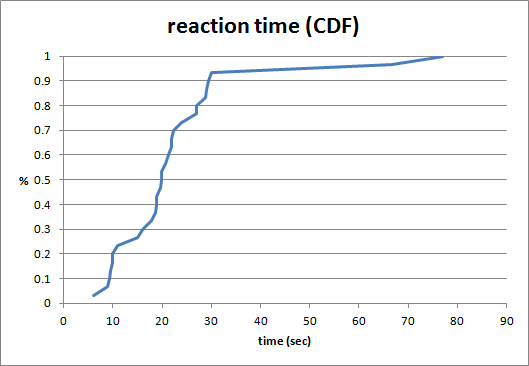
\includegraphics[width=\columnwidth]{reaction_cdf.PNG}
\end{figure*}

\end{document}
